\documentclass[10pt]{article}

\usepackage{amsmath}
\usepackage{graphicx}
\usepackage[margin=0.7in]{geometry}
\usepackage{float}
\usepackage{listings}
\usepackage[utf8]{inputenc}
\usepackage[parfill]{parskip}  
\usepackage{multicol}
\usepackage{siunitx}
\usepackage[dvipsnames]{xcolor}
% \usepackage{hyperref}
\usepackage{cleveref}
\usepackage{cite}
\usepackage{caption}
\usepackage{tabularx}
\usepackage{mathabx}
\usepackage{titling}

\captionsetup{width=0.6\linewidth}

\newcommand{\rhomax}{\rho_{\text{max}}}
\newcommand{\relerr}{\epsilon_{\text{rel}}}
\newcommand{\bigO}[1]{\mathcal{O}(#1)}

\graphicspath{{../results/}}

\newcommand\myshade{50}
\colorlet{mylinkcolor}{violet}
\colorlet{mycitecolor}{YellowOrange}
\colorlet{myurlcolor}{Aquamarine}


\begin{document}
\title{Molecular Dynamics
\\ Project 5
\\ FYS3150}
\author{Ragnar Bruvoll \and Halvard Sutterud}
%\author{Halvard Sutterud}
\date{November 2017}
\maketitle{\begin{center}\end{center}}
\pagenumbering{gobble}
\thispagestyle{empty}

\begin{figure}[htpb]
    \centering
    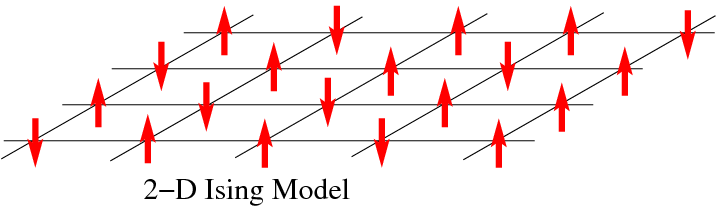
\includegraphics[width=0.8\linewidth]{../results/front.png}
    \label{fig:name}
\end{figure}

\begin{abstract}
    The aim of this report is to educate the reader on the subject of molecular dynamis. We will use \texttt{c++} to create a model and a program called \texttt{ovito} to visualize it.
\end{abstract}

\newpage



\begin{multicols}{2}
\tableofcontents

% \newpage
\pagenumbering{arabic}
%%%%%%%%%%%%%%%%%%%%%%%%%%%%%%%%%%%%%%%%%%%%%%%%%%%%%%%%%%
\section{Introduction}
Our simulation consists of a number of argon atoms placed uniformly inside a cube with side lengths of 10 angstroms. The atoms behave according to Maxwell-Boltzmann distrubution
\begin{align} 
P(v_i)d\mathrm{v}_i = \left(\frac{m}{2\pi k_B
T}\right)^{1/2} \exp\left(-\frac{m v_i^2}{2k_B T}\right)d\mathrm{v}_i,
\end{align} 
which will be described in detail in the next section


%%%%%%%%%%%%%%%%%%%%%%%%%%%%%%%%%%%%%%%%%%%%%%%%%%%%%%%%%%
\section{Theory}
\subsection{Maxwell-Boltzmann distrubution}
\begin{align} 
P(v_i)d\mathrm{v}_i = \left(\frac{m}{2\pi k_B
T}\right)^{1/2} \exp\left(-\frac{m v_i^2}{2k_B T}\right)d\mathrm{v}_i,
\end{align} 

\subsection{Random particles}
\subsection{Particles in box}
\subsection{Face-centered cubic lattice}
\subsection{Forces}
\subsection{Energies}
\subsection{Diffusion}


%%%%%%%%%%%%%%%%%%%%%%%%%%%%%%%%%%%%%%%%%%%%%%%%%%%%%%%%%%
\section{Methods}
\subsection{Setting up the system}
\subsection{Making periodic boundry conditions and zero total momentum}
\subsection{Calculating forces}
\subsection{Calculating energies}



%%%%%%%%%%%%%%%%%%%%%%%%%%%%%%%%%%%%%%%%%%%%%%%%%%%%%%%%%%
\section{Results}


%%%%%%%%%%%%%%%%%%%%%%%%%%%%%%%%%%%%%%%%%%%%%%%%%%%%%%%%%%
\section{Discussion and conclusions}





\bibliography{bib1}{}
\bibliographystyle{plain}

\end{multicols}


\end{document}
